% Author: Izaak Neutelings (Februari, 2020)

\documentclass[border=3pt,tikz]{standalone}
\usepackage{amsmath} % for \dfrac
\usepackage{bm}
\usepackage{physics}
\usepackage{tikz,pgfplots}
\usepackage[outline]{contour} % glow around text
\usetikzlibrary{angles,quotes} % for pic (angle labels)
\usetikzlibrary{decorations.markings}
\usetikzlibrary{calc}
\usetikzlibrary{shapes,intersections} % for path name
\tikzset{>=latex} % for LaTeX arrow head
\contourlength{1.4pt}

\usepackage{xcolor}
\colorlet{Ecol}{orange!90!black}
\colorlet{EcolFL}{orange!90!black}
\colorlet{veccol}{green!45!black}
\colorlet{EFcol}{red!60!black}
\colorlet{veccol}{green!45!black}
\colorlet{Icol}{blue!70!black}
\colorlet{Ampcol}{green!60!black!70}
\colorlet{gausscol}{green!50!black!80}
\tikzstyle{current}=[->,Icol,thick]
\colorlet{pluscol}{red!60!black}
\colorlet{minuscol}{blue!60!black}
\tikzstyle{anode}=[top color=red!20,bottom color=red!50,shading angle=20]
\tikzstyle{cathode}=[top color=blue!20,bottom color=blue!40,shading angle=20]
\tikzstyle{gauss surf}=[green!40!black,top color=green!2,bottom color=green!80!black!70,shading angle=5,fill opacity=0.4]
\tikzstyle{metal}=[top color=black!15,bottom color=black!25,middle color=black!20,shading angle=10]
\tikzstyle{vector}=[->,thick,veccol]
\tikzstyle{Cstyle}=[very thick,orange!90!black]
\tikzstyle{EField}=[->,thick,Ecol]
\tikzstyle{EField dashed}=[dashed,Ecol,line width=0.6]
\tikzstyle{mydashes}=[dash pattern=on 1 off 1]
\tikzset{
  EFieldLine/.style={thick,EcolFL,decoration={markings,
                     mark=at position #1 with {\arrow{latex}}},
                     postaction={decorate}},
  EFieldLine/.default=0.5}



\begin{document}


% CAPACITOR 2D
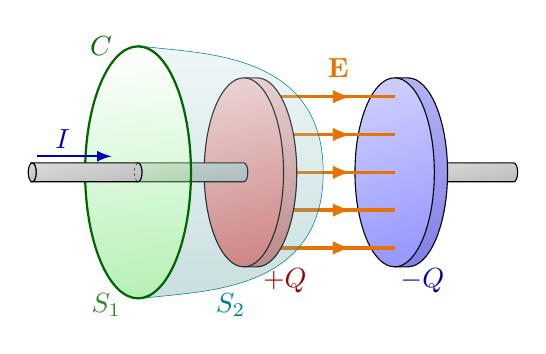
\begin{tikzpicture}[xscale=0.42]
  
  \def\RC{1.2}
  \def\RW{0.1*\RC}
  \def\RA{1.6}
  \def\D{2.6*\RA}
  \def\T{0.4}
  \def\L{2*\RA}
  \def\NE{5}
  %\def\NQ{7}
  
  % CATHODE WIRE
  \draw[metal]
    (\D+\T,\RW) --++ (\L,0) arc (90:-90:\RW) --++ (-\L,0);
  
  % CATHODE
  \draw[cathode,top color=blue!90!black!30,bottom color=blue!80!black!50]
    (\D,\RC) --++ (\T,0) arc (90:-90:\RC) --++ (-\T,0);
  \draw[cathode] (\D,0) circle (\RC);
  
  % ELECTRIC FIELD
  \foreach \i [evaluate={\y=-\RC+(\i-0.5)*(2*\RC)/\NE);}] in {1,...,\NE}{
    \draw[EFieldLine={0.68},very thick] (0,\y) --++ (\D,0);
  }
  \node[Ecol,above] at (0.59*\D,0.9*\RC) {$\vb{E}$};
  
  % ANODE
  \draw[anode,top color=red!90!black!20,bottom color=red!80!black!50]
    (-\T,\RC) --++ (\T,0) arc (90:-90:\RC) --++ (-\T,0);
  \draw[anode] (-\T,0) circle (\RC);
  %\foreach \i [evaluate={\y=(\i-0.5)*\H/\NQ;}] in {1,...,\NQ}{
  %  \node[pluscol,scale=0.9] at (-\w/2,\y) {$+$};
  %  \node[minuscol,scale=0.9] at (\W+\w/2,\y) {$-$};
  %}
  
  % ANODE WIRE LEFT
  \draw[metal]
    (-\T,\RW) arc (90:-90:\RW) --++ (-\L,0) arc (-90:90:\RW) -- cycle;
  
  % SURFACE
  \draw[gauss surf,very thin,fill opacity=0.3,green!50!blue,top color=green!50!blue!20,bottom color=green!50!blue!80!black!70]
    %(-\T-\L,\RA) arc (90:-90:{1.2*(\T+\L+\RA)} and {\RA}) arc (-90:90:\RA);
    (-\T-\L,1.006*\RA) to[out=-4,in=90,looseness=0.7] (\T+\RA,0) to[out=-90,in=4,looseness=0.7] (-\T-\L,-1.006*\RA) arc (-90:90:1.006*\RA);
  \draw[gauss surf,thick]
    (-\T-\L,0) circle (\RA);
  \node[green!40!black] at (-\T-\L-0.7*\RA,\RA) {$C$};
  \node[green!40!black!80] at (-\T-\L-0.6*\RA,-1.05*\RA) {$S_1$};
  \node[green!50!blue] at (-0.5*\RA,-1.05*\RA) {$S_2$};
  \node[pluscol] at (0.7*\RC,-1.15*\RC) {$+Q$};
  \node[minuscol] at (\D+0.7*\RC,-1.15*\RC) {$-Q$};
  
  % ANODE WIRE RIGHT
  \draw[metal]
    (-\T-\L,\RW) arc (90:-90:\RW) --++ (-\L,0) arc (-90:90:\RW) -- cycle;
  \draw[mydashes,black!80,very thin]
    (-\T-\L,0.94*\RW) arc (90:270:0.94*\RW);
  \draw[metal]
    (-\T-2*\L,0) circle (\RW);
  \draw[current] (-\T-1.95*\L,1.7*\RW) --++ (0.7*\L,0) node[midway,right=1,above left=-1] {$I$};
  
  %\node[pluscol] at (-2.1*\w,\H) {$+Q$};
  %\node[minuscol] at (\W+2.1*\w,\H) {$-Q$};
  
\end{tikzpicture}



\end{document}
